\chapter{\ifenglish Background Knowledge and Theory\else ทฤษฎีที่เกี่ยวข้อง\fi}


\section{การแบ่งส่วนภาพ (Image Segmentation)}
การแบ่งส่วนภาพ (Image Segmentation) เป็นกระบวนการสำคัญในงานประมวลผลภาพดิจิทัล โดยมีวัตถุประสงค์เพื่อแยกภาพออกเป็นส่วนย่อย ๆ หรือบริเวณ (regions) ที่มีความหมาย เพื่อให้ง่ายต่อการวิเคราะห์ในขั้นตอนถัดไป โดยทั่วไป การแบ่งส่วนภาพจะทำการจัดกลุ่มพิกเซลที่มีลักษณะคล้ายคลึงกัน เช่น สี ความเข้ม หรือพื้นผิว ให้อยู่ในกลุ่มเดียวกัน

การแบ่งส่วนภาพสามารถแบ่งออกได้เป็นหลายประเภท โดยประเภทที่นิยมในงานด้านปัญญาประดิษฐ์ ได้แก่ การแบ่งส่วนภาพเชิงความหมาย (Semantic Segmentation) ซึ่งเป็นการจำแนกประเภทให้กับพิกเซลในภาพว่าเป็นประเภทใด เช่น การระบุว่าแต่ละพิกเซลเป็นส่วนของอวัยวะใดในช่องปาก การแบ่งส่วนภาพเชิงวัตถุ (Instance Segmentation) คือ การแบ่งส่วนวเฉพาะวัตถุที่สนใจที่อาจปรากฏหลายวัตถุในภาพเดียวกัน เช่น ในภาพเดียวกันมีคนอยู่หลายคน การแบ่งส่วนแบบ Instance จะแยกคนแตต่ละคนออกจากกัน 
และการแบ่งส่วนภาพแบบ Panoptic เป็นการแบ่งส่วนแบบรวม Semantic และ Instance เข้าด้วยกัน โดยมีเป้าหมายเพื่อระบุประเภทของพิกเซลทุกพิกเซลในภาพ ซึ่งกำหนดให้พิกเซลที่อยู่ในกลุ่ม "Stuff" (พื้นหลังที่นับจำนวนไม่ได้ เช่น ถนน, ท้องฟ้า) ถูกจำแนกตามประเภทของข้อมูล และพิกเซลที่อยู่ในกลุ่ม "Things" (วัตถุที่นับจำนวนได้ เช่น คน, รถยนต์) ถูกจำแนกทั้งประเภทและแยกแยะวัตถุออกจากกันอย่างชัดเจน \cite{minaee2021survey}

ในบริบทของงานทางการแพทย์ การแบ่งส่วนภาพมีบทบาทสำคัญในการระบุขอบเขตของอวัยวะหรือรอยโรค ซึ่งช่วยให้สามารถประเมินลักษณะ ขนาด และตำแหน่งของความผิดปกติได้อย่างแม่นยำมากขึ้น \cite{medical_image_segmentation} อย่างไรก็ตาม ภาพทางการแพทย์มักมีความซับซ้อนและแตกต่างกันในแต่ละบุคคล รวมถึงอาจมีสัญญาณรบกวน (noise) ซึ่งส่งผลต่อความยากในการแบ่งส่วนภาพ

ในอดีต อัลกอริทึมแบบดั้งเดิม เช่น Otsu thresholding, Watershed transform และ Active contour ถูกนำมาใช้อย่างแพร่หลายในงานแบ่งส่วนภาพทางการแพทย์ อย่างไรก็ตาม ในช่วงไม่กี่ปีที่ผ่านมา การเรียนรู้เชิงลึก (Deep Learning) ได้เข้ามามีบทบาทสำคัญ เนื่องจากสามารถให้ผลลัพธ์ที่มีความแม่นยำสูงกว่าในหลายงานวิจัย \cite{minaee2021survey}

\begin{figure}[H]
  \centering
  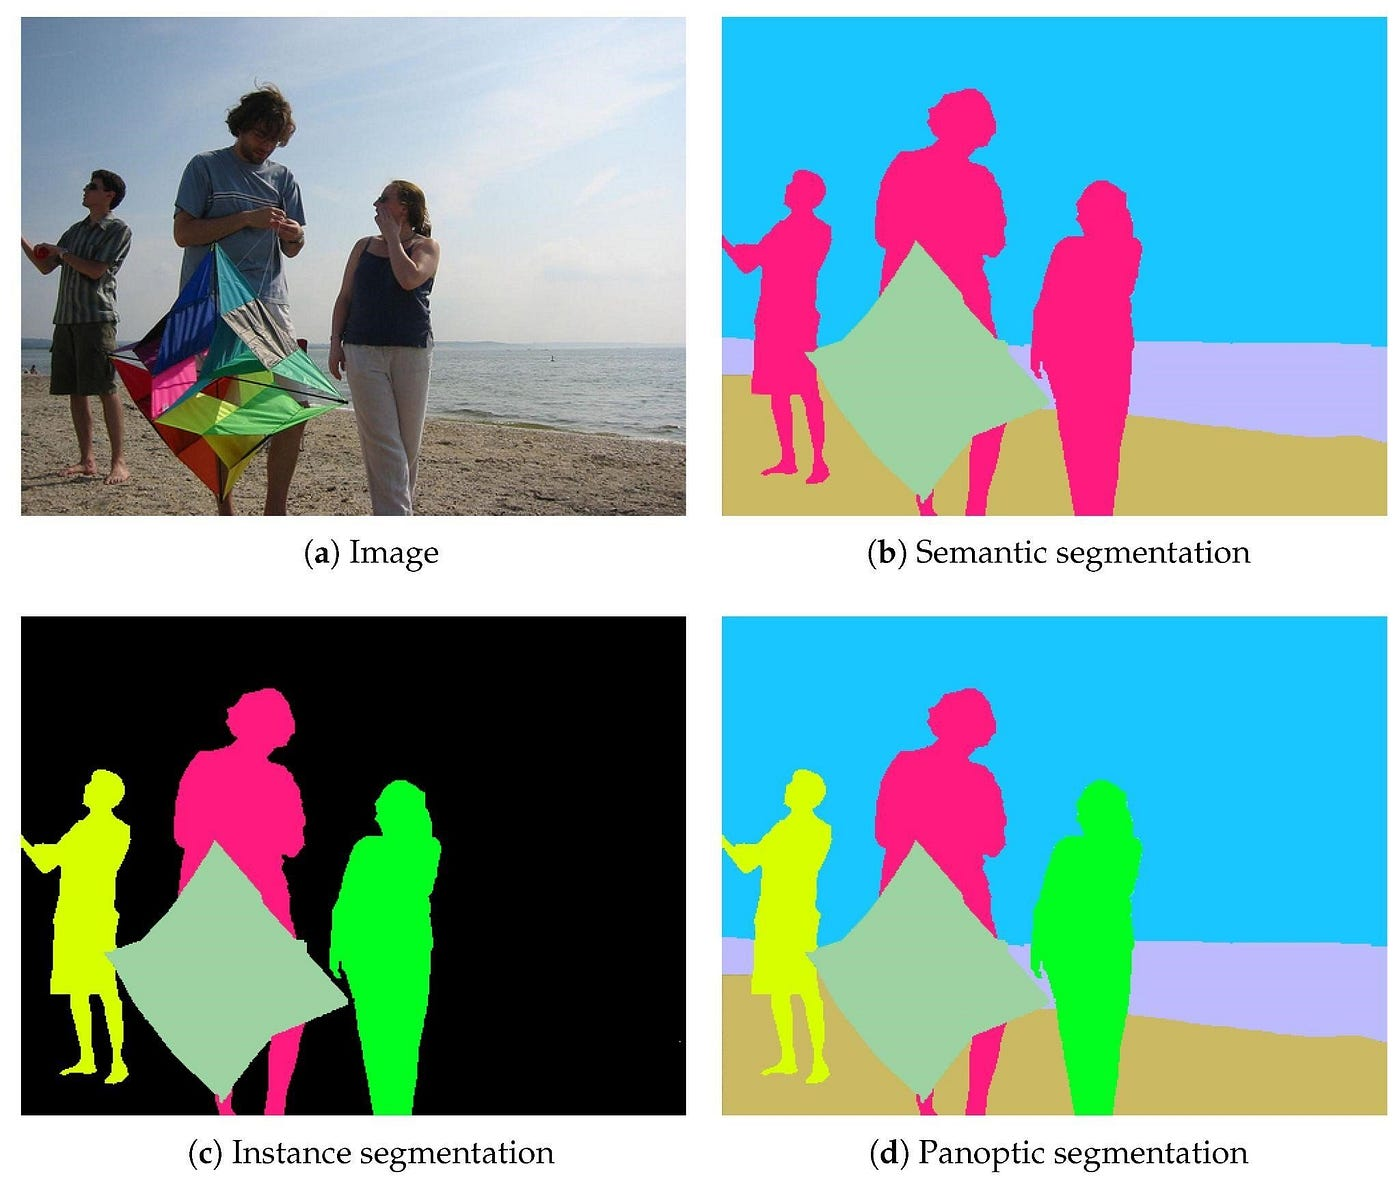
\includegraphics[width=0.45\textwidth]{images/segmentation_types.jpg}
  \caption{ตัวอย่างภาพแสดงประเภทของการแบ่งส่วนภาพ ได้แก่ Semantic Segmentation, Instance Segmentation และ Panoptic Segmentation \cite{minaee2021survey}}
  \label{fig:segmentation-types}
\end{figure}


\section{Convolutional Neural Network (CNN)}
Convolutional Neural Network (CNN) เป็นหนึ่งในสถาปัตยกรรมหลักของโครงข่ายประสาทเทียมในการเรียนรู้เชิงลึก (Deep Learning) ที่ถูกออกแบบมาเพื่อประมวลผลข้อมูลที่มีโครงสร้างเชิงพื้นที่ เช่น ภาพและวิดีโอ โดยมีจุดเด่นในการเรียนรู้คุณลักษณะ (features) จากข้อมูลได้โดยอัตโนมัติผ่านกระบวนการ convolution ซึ่งใช้ตัวกรอง (filters หรือ kernels) ในการตรวจจับลักษณะสำคัญของภาพ เช่น ขอบ (edges), มุม (corners) และรูปแบบเชิงซับซ้อนในระดับที่ลึกขึ้น \cite{krizhevsky2012imagenet, lecun2015deep}

โครงสร้างพื้นฐานของ CNN ประกอบด้วยหลายชั้น (layers) ได้แก่ convolutional layer, activation function (เช่น ReLU), pooling layer และ fully connected layer โดย convolutional layer ทำหน้าที่สกัดคุณลักษณะจากภาพอินพุต (Input) ในขณะที่ pooling layer ช่วยลดขนาดของข้อมูล (downsampling) เพื่อลดความซับซ้อนและป้องกัน overfitting ส่วน activation function ช่วยเพิ่มความไม่เป็นเชิงเส้นให้กับโมเดล ทำให้สามารถเรียนรู้ความสัมพันธ์ที่ซับซ้อนได้ \cite{goodfellow2016deep}
นอกจากนี้ CNN ยังมีคุณสมบัติสำคัญ เช่น local connectivity และ weight sharing ซึ่งช่วยลดจำนวนพารามิเตอร์ของโมเดลเมื่อเทียบกับโครงข่ายแบบ fully connected และทำให้สามารถเรียนรู้ได้อย่างมีประสิทธิภาพมากขึ้นในงานที่เกี่ยวข้องกับภาพ \cite{lecun2015deep}

ในงานด้านการแบ่งส่วนภาพ CNN มักถูกนำมาใช้ในรูปแบบของ fully convolutional network (FCN) ซึ่งแทนที่ fully connected layer ด้วย convolutional layer ทั้งหมด เพื่อให้สามารถสร้างผลลัพธ์ในระดับพิกเซล (pixel-wise prediction) ได้ \cite{long2015fcn} โดยโครงสร้างแบบ encoder-decoder เช่น U-Net และ DeepLabV3+ เป็นการต่อยอดจากแนวคิดของ CNN เพื่อรักษาข้อมูลเชิงตำแหน่ง (spatial information) และเพิ่มความแม่นยำในการแบ่งส่วนภาพ \cite{chen2018deeplab,ronneberger2015unet}

\begin{figure}[H]
  \centering
  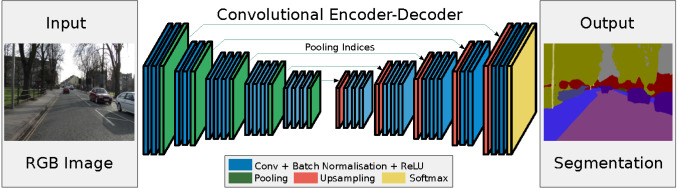
\includegraphics[width=0.8\textwidth]{images/cnn.jpg}
  \caption{โครงสร้างพื้นฐานของ Convolutional Neural Network (CNN) ที่ประกอบด้วย convolutional layer, activation function, pooling layer และ fully connected layer \cite{goodfellow2016deep}}
  \label{fig:cnn-architecture}
\end{figure}

\section{แบบจำลองสำหรับการแบ่งส่วนภาพ (Segmentation Models)}
\subsection{U-Net}
U-Net เป็นแบบจำลองการแบ่งส่วนภาพที่ถูกออกแบบมาสำหรับงานทางการแพทย์โดยเฉพาะ โดยมีโครงสร้างแบบ encoder-decoder ที่มีลักษณะสมมาตร (symmetric architecture) ซึ่งประกอบด้วยส่วน encoder สำหรับลดขนาดของภาพและสกัดคุณลักษณะ และส่วน decoder สำหรับเพิ่มความละเอียดของภาพและสร้าง segmentation mask \cite{ronneberger2015unet}

จุดเด่นสำคัญของ U-Net คือการใช้ skip connections ซึ่งเชื่อมต่อ feature map จาก encoder ไปยัง decoder ในระดับที่สอดคล้องกัน ช่วยให้โมเดลสามารถรักษาข้อมูลเชิงตำแหน่ง (spatial information) และรายละเอียดของขอบวัตถุได้ดีขึ้น ส่งผลให้มีประสิทธิภาพสูงในการแบ่งส่วนภาพที่ต้องการความละเอียด เช่น ภาพทางการแพทย์
นอกจากนี้ U-Net ยังสามารถฝึกด้วยข้อมูลจำนวนน้อยได้ดีเมื่อเทียบกับโมเดลอื่น เนื่องจากมีการใช้ data augmentation และโครงสร้างที่เหมาะสมกับลักษณะของภาพทางการแพทย์

\begin{figure}[H]
  \centering
  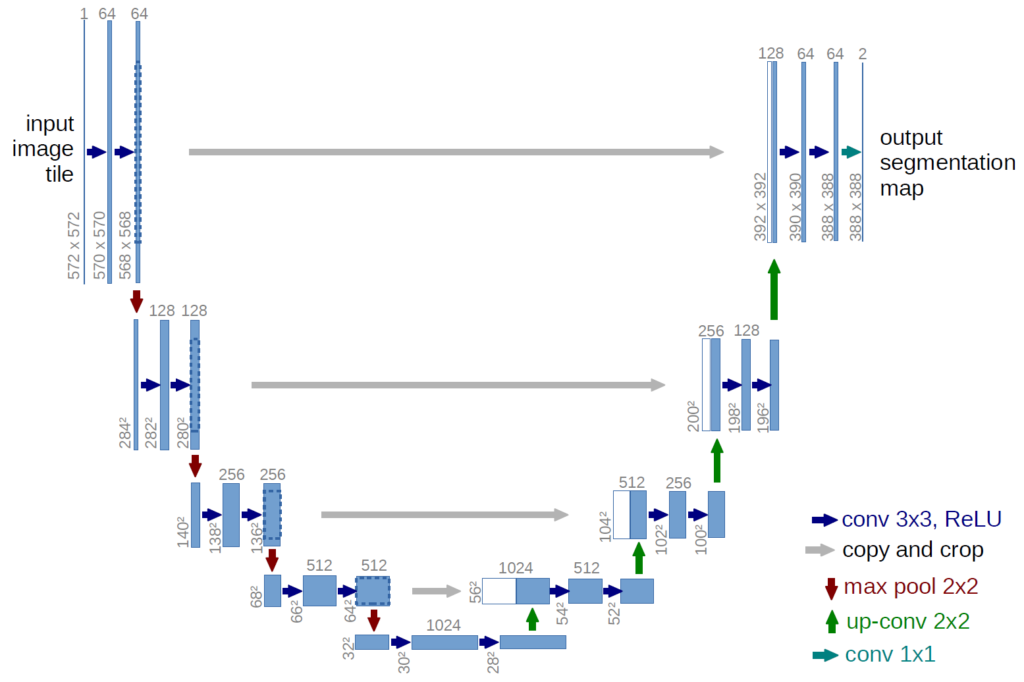
\includegraphics[width=0.5\textwidth]{images/unet.png}
  \caption{โครงสร้างของ U-Net ซึ่งประกอบด้วยส่วน encoder และ decoder ที่เชื่อมต่อกันด้วย skip connections \cite{ronneberger2015unet}}
  \label{fig:unet-architecture}
\end{figure}


\subsection{LinkNet}
LinkNet เป็นแบบจำลอง segmentation ที่พัฒนาขึ้นโดยเน้นประสิทธิภาพในการประมวลผลและความเร็ว โดยมีโครงสร้างแบบ encoder-decoder เช่นเดียวกับ U-Net แต่มีการออกแบบให้ lightweight มากขึ้น \cite{chaurasia2017linknet}
ใน LinkNet จะมีการเชื่อมต่อระหว่าง encoder และ decoder ผ่าน residual connections ซึ่งช่วยให้ข้อมูลสามารถไหลผ่านเครือข่ายได้อย่างมีประสิทธิภาพ และลดปัญหา gradient vanishing นอกจากนี้ LinkNet ยังมีจำนวนพารามิเตอร์น้อย ทำให้เหมาะสำหรับการใช้งานที่ต้องการความเร็วสูงหรือมีข้อจำกัดด้านทรัพยากร
โมเดลนี้มักใช้ร่วมกับ encoder ที่มีประสิทธิภาพ เช่น ResNet หรือ MobileNet เพื่อเพิ่มความสามารถในการสกัดคุณลักษณะจากภาพ (Feature Extraction) และยังคงรักษาความเร็วในการประมวลผลที่ดี

\begin{figure}[H]
  \centering
  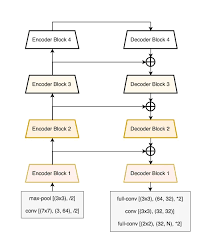
\includegraphics[width=0.4\textwidth]{images/linknet.png}
  \caption{โครงสร้างของ LinkNet ที่มีการเชื่อมต่อแบบ residual connections ระหว่าง encoder และ decoder \cite{chaurasia2017linknet}}
  \label{fig:linknet-architecture}
\end{figure}



\subsection{DeepLabV3+}
DeepLabV3+ เป็นแบบจำลอง segmentation ที่พัฒนาขึ้นเพื่อเพิ่มความสามารถในการจับบริบทของภาพ (context) และรายละเอียดของขอบวัตถุ โดยใช้เทคนิค atrous convolution (หรือ dilated convolution) ซึ่งช่วยเพิ่ม receptive field โดยไม่เพิ่มจำนวนพารามิเตอร์ \cite{chen2018deeplab}
โครงสร้างของ DeepLabV3+ ประกอบด้วยส่วน encoder ที่ใช้ atrous spatial pyramid pooling (ASPP) เพื่อดึงข้อมูลในหลายสเกล และส่วน decoder ที่ช่วยปรับปรุงความละเอียดของขอบวัตถุให้คมชัดมากขึ้น

จุดเด่นของโมเดลนี้ คือ สามารถจัดการกับวัตถุที่มีขนาดแตกต่างกันในภาพเดียว และรักษารายละเอียดของ segmentation ได้ดี ทำให้ได้รับความนิยมในงาน segmentation ที่ต้องการความแม่นยำสูง

\begin{figure}[H]
  \centering
  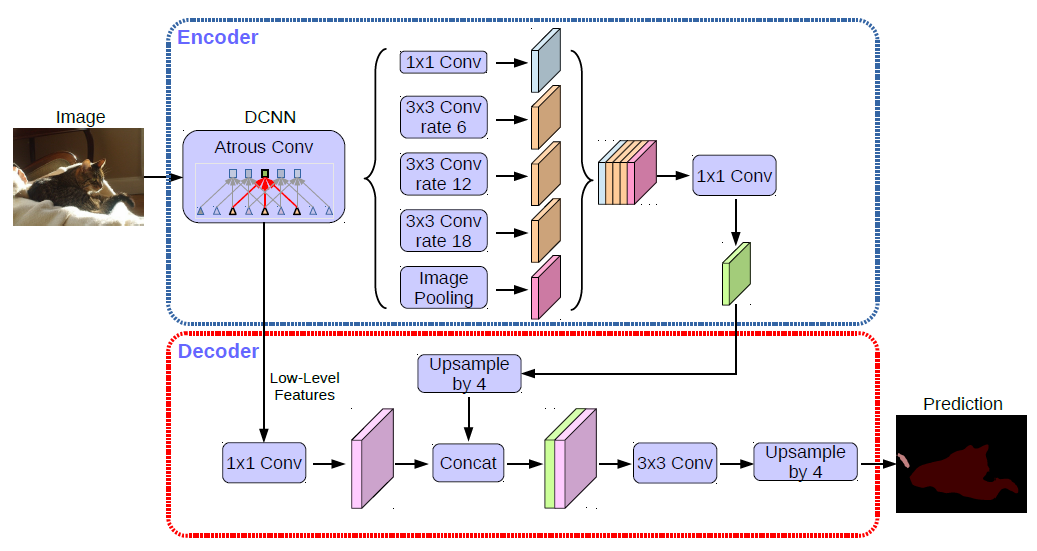
\includegraphics[width=0.8\textwidth]{images/deeplabv3+.png}
  \caption{โครงสร้างของ DeepLabV3+ ที่ใช้ atrous convolution และ ASPP เพื่อเพิ่มความสามารถในการจับบริบทของภาพ \cite{chen2018deeplab}}
  \label{fig:deeplabv3plus-architecture}
\end{figure}


\subsection{UPerNet}
UPerNet (Unified Perceptual Parsing Network) เป็นแบบจำลอง segmentation ที่ออกแบบมาเพื่อรวมข้อมูลจากหลายระดับของ feature (multi-scale features) โดยใช้โครงสร้างที่ผสาน Feature Pyramid Network (FPN) และ Pyramid Pooling Module (PPM) เข้าด้วยกัน \cite{xiao2018upernet}

โดยที่ UPerNet มีการใช้ FPN เพื่อรวมข้อมูลจากหลายระดับของ feature map ซึ่งช่วยให้โมเดลสามารถจับบริบทของภาพได้ดีขึ้น ในขณะที่ PPM ช่วยให้โมเดลสามารถรวมข้อมูลจากหลายสเกลได้อย่างมีประสิทธิภาพ ทำให้สามารถจัดการกับวัตถุที่มีขนาดแตกต่างกันในภาพเดียวกันได้ดีขึ้น

UPerNet สามารถรวมข้อมูลทั้งในระดับ global context และ local detail ได้อย่างมีประสิทธิภาพ ทำให้สามารถจัดการกับภาพที่มีความซับซ้อนและมีวัตถุหลายขนาดได้ดี นอกจากนี้ยังสามารถนำไปประยุกต์ใช้กับงาน segmentation ที่ต้องการความละเอียดสูงและความเข้าใจเชิงบริบทของภาพ

\begin{figure}[H]
  \centering
  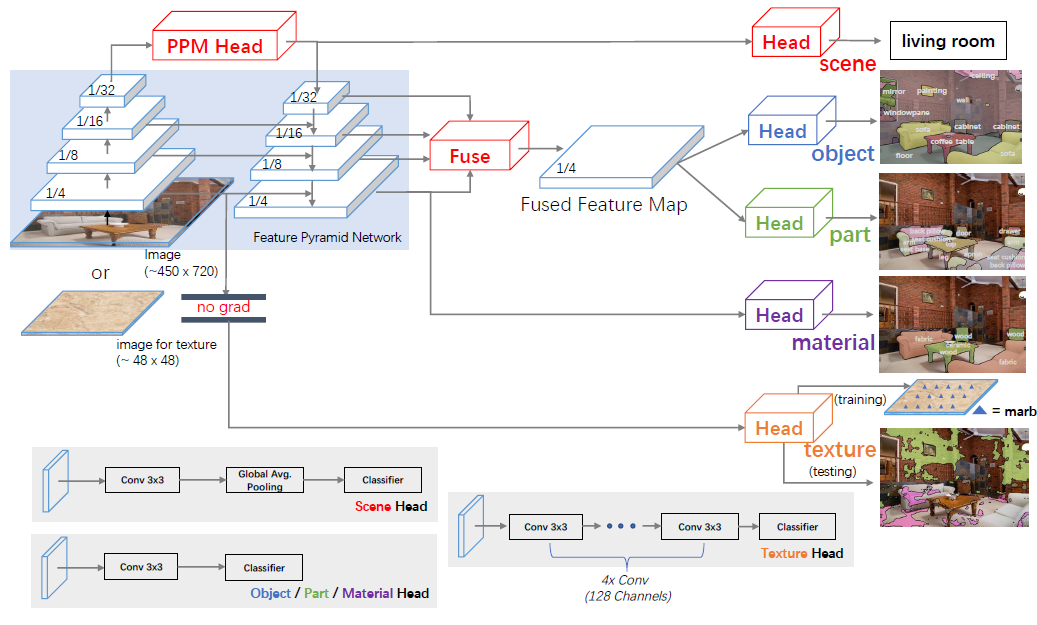
\includegraphics[width=0.6\textwidth]{images/upernet.png}
  \caption{โครงสร้างของ UPerNet ที่ผสาน FPN และ PPM เพื่อรวมข้อมูลจากหลายระดับของ feature map \cite{xiao2018upernet}}
  \label{fig:upernet-architecture}
\end{figure}


\section{Encoder / Backbone}
Encoder หรือ Backbone เป็นส่วนสำคัญของแบบจำลองการแบ่งส่วนภาพ ทำหน้าที่สกัดคุณลักษณะ (feature extraction) จากภาพอินพุต (Input) โดยทั่วไปจะใช้โครงข่ายที่ผ่านการฝึกสอนมาก่อน (pretrained models) บนชุดข้อมูลขนาดใหญ่ เช่น ImageNet เพื่อช่วยให้โมเดลสามารถเรียนรู้ลักษณะสำคัญของภาพได้อย่างมีประสิทธิภาพมากขึ้น \cite{he2016resnet, sandler2018mobilenetv2, tan2019efficientnet}

\subsection{ResNet50 และ ResNet101}
ResNet (Residual Network) เป็นโครงข่ายประสาทเทียมที่พัฒนาเพื่อแก้ปัญหา vanishing gradient ในเครือข่ายที่มีความลึกมาก โดยใช้แนวคิด residual learning ซึ่งมีการเพิ่ม shortcut connection หรือ skip connection ระหว่างชั้น เพื่อให้โมเดลสามารถเรียนรู้ส่วนที่เหลือ (residual) ของข้อมูลแทนที่จะเรียนรู้ mapping ทั้งหมด \cite{he2016resnet}

ResNet50 และ ResNet101 แตกต่างกันที่จำนวนชั้น โดย ResNet50 มีประมาณ 50 ชั้น และ ResNet101 มีประมาณ 101 ชั้น ซึ่งทำให้ ResNet101 สามารถเรียนรู้คุณลักษณะที่ซับซ้อนมากขึ้น แต่ต้องใช้ทรัพยากรในการประมวลผลสูงกว่า
จุดเด่นของ ResNet อยู่ที่ความสามารถในการเรียนรู้ feature เชิงลึกได้ดี และมีความเสถียรในการฝึก ทำให้ถูกนำมาใช้เป็น backbone ในงาน segmentation อย่างแพร่หลาย เช่น DeepLabV3+ และ UPerNet

\subsection{MobileNetV2}
MobileNetV2 เป็นโครงข่ายที่ออกแบบมาเพื่อให้มีขนาดเล็กและมีประสิทธิภาพสูง เหมาะสำหรับอุปกรณ์ที่มีข้อจำกัดด้านทรัพยากร โดยใช้แนวคิด inverted residual structure และ linear bottleneck ซึ่งช่วยลดจำนวนพารามิเตอร์และการคำนวณลงอย่างมาก \cite{sandler2018mobilenetv2}

โครงสร้าง inverted residual จะเริ่มจากการขยายมิติของ feature (expansion) จากนั้นทำ depthwise convolution และลดมิติกลับ (projection) ทำให้สามารถรักษาข้อมูลสำคัญได้ในขณะที่ลดความซับซ้อนของโมเดล
MobileNetV2 จึงเหมาะสำหรับงานที่ต้องการความเร็ว เช่น real-time processing หรือระบบที่มีข้อจำกัดด้านหน่วยความจำ


\subsection{EfficientNet-B3 และ EfficientNet-B7}
EfficientNet เป็นโครงข่ายที่พัฒนาขึ้นเพื่อเพิ่มประสิทธิภาพของโมเดลโดยใช้แนวคิด compound scaling ซึ่งปรับขนาดของโมเดลในสามมิติ ได้แก่ ความลึก (depth), ความกว้าง (width) และความละเอียดของภาพ (resolution) อย่างสมดุล \cite{tan2019efficientnet}
EfficientNet-B3 และ EfficientNet-B7 เป็นเวอร์ชันที่มีขนาดแตกต่างกัน โดย:
\begin{itemize}
  \item EfficientNet-B3 มีขนาดกลาง ให้สมดุลระหว่างความแม่นยำและความเร็ว
  \item EfficientNet-B7 มีขนาดใหญ่ ให้ความแม่นยำสูง แต่ใช้ทรัพยากรสูงมาก
\end{itemize}
EfficientNet เด่นด้านการใช้พารามิเตอร์อย่างมีประสิทธิภาพ ทำให้สามารถให้ผลลัพธ์ที่ดีในขณะที่ใช้ทรัพยากรน้อยกว่าโมเดลแบบดั้งเดิม


\section{Loss Function}
ในการฝึกแบบจำลองการแบ่งส่วนภาพ (image segmentation) ฟังก์ชันการสูญเสีย (loss function) มีบทบาทสำคัญในการวัดความแตกต่างระหว่างผลลัพธ์ที่แบบจำลองทำนาย (prediction) และข้อมูลจริง (ground truth) เพื่อปรับปรุงพารามิเตอร์ของโมเดลให้มีความแม่นยำมากขึ้น โดยในงานนี้เลือกใช้ Dice Loss และ Cross-Entropy Loss ซึ่งเป็นฟังก์ชันที่นิยมใช้ในงาน segmentation ทางการแพทย์ \cite{milletari2016vnet, sudre2017dice}

\subsection{Dice Loss}
Dice Loss เป็นฟังก์ชันที่พัฒนามาจาก Dice Coefficient ซึ่งใช้วัดความสอดคล้องระหว่าง prediction และ ground truth โดยมีค่าอยู่ระหว่าง 0 ถึง 1 ซึ่งค่าที่สูงแสดงถึงความสอดคล้องที่ดี โดยสามารถนิยาม Dice Coefficient ได้ดังนี้
\begin{equation}
\text{Dice} = 1 - \frac{2 \sum_{i=1}^{N} p_i g_i + \epsilon}{\sum_{i=1}^{N} p_i + \sum_{i=1}^{N} g_i + \epsilon}
\end{equation}
โดยที่ $p_i$ คือค่าที่โมเดลทำนายสำหรับพิกเซลที่ $i$, $g_i$ คือค่าจริงของพิกเซลที่ $i$, และ $\epsilon$ เป็นค่าคงที่เล็ก ๆ เพื่อป้องกันการหารด้วยศูนย์

Dice Loss มีจุดเด่นด้านความสามารถในการจัดการกับปัญหา class imbalance ซึ่งมักพบในงาน segmentation ทางการแพทย์ เช่น กรณีที่พื้นที่ของรอยโรคมีขนาดเล็กเมื่อเทียบกับพื้นหลัง \cite{milletari2016vnet} นอกจากนี้ยังช่วยให้โมเดลเรียนรู้ขอบเขตของวัตถุได้ดีขึ้น
ทว่า Dice Loss อาจมีความไม่เสถียรในช่วงเริ่มต้นของการฝึก เนื่องจากค่าของตัวหารอาจมีค่าน้อยมากในบางกรณี

\subsection{Cross-Entropy Loss}
Cross-Entropy Loss เป็นฟังก์ชันที่นิยมใช้ในงาน classification และสามารถนำมาประยุกต์ใช้ในงาน segmentation ได้ โดยทำการคำนวณความแตกต่างระหว่าง probability distribution ของ prediction และ ground truth โดยสำหรับกรณี binary segmentation สามารถนิยามได้ดังนี้
\begin{equation}
\mathcal{L}_{MCE} = -\frac{1}{N} \sum_{i=1}^{N} \sum_{c=1}^{C} g_{ic} \log(p_{ic})
\end{equation}
โดยที่ $N$ คือจำนวนพิกเซลทั้งหมด, $C$ คือจำนวนคลาส, $g_{ic}$ คือค่าจริงของพิกเซลที่ $i$ สำหรับคลาส $c$, และ $p_{ic}$ คือค่าที่โมเดลทำนายสำหรับพิกเซลที่ $i$ สำหรับคลาส $c$

ข้อดีของ Cross-Entropy Loss คือความเสถียรในการฝึก และความสามารถในการทำให้โมเดลเรียนรู้การจำแนกพิกเซลได้อย่างมีประสิทธิภาพ อย่างไรก็ตาม ฟังก์ชันนี้อาจมีข้อจำกัดในกรณีที่ข้อมูลมี class imbalance เนื่องจากพิกเซลของคลาสใหญ่จะมีอิทธิพลต่อค่าความสูญเสียมากกว่า \cite{goodfellow2016deep}


\subsection{การใช้งานร่วมกันของ Dice Loss และ Cross-Entropy Loss}
ในงาน segmentation หลายงานนิยมใช้ Dice Loss และ Cross-Entropy Loss ร่วมกัน เพื่อรวมข้อดีของทั้งสองฟังก์ชัน โดย Cross-Entropy Loss ช่วยให้โมเดลเรียนรู้การจำแนกพิกเซลได้อย่างเสถียร ในขณะที่ Dice Loss ช่วยปรับปรุงความแม่นยำของขอบเขตวัตถุและลดผลกระทบจาก class imbalance \cite{sudre2017dice}

สำหรับโครงงานนี้ การใช้ loss function ทั้งสองร่วมกันช่วยให้แบบจำลองสามารถให้ผลลัพธ์ที่มีความแม่นยำมากขึ้น โดยเฉพาะในกรณีที่รอยโรคมีขนาดเล็กหรือมีลักษณะไม่สม่ำเสมอ ซึ่งสอดคล้องกับลักษณะของข้อมูลภาพช่องปากที่ใช้ในการทดลอง


\section{การประมวลผลข้อมูลขั้นต้น (Preprocessing)}
Preprocessing เป็นขั้นตอนสำคัญในการเตรียมข้อมูลก่อนนำเข้าสู่แบบจำลอง โดยมีวัตถุประสงค์เพื่อปรับปรุงคุณภาพของข้อมูล ลดสัญญาณรบกวน (noise) และทำให้ข้อมูลมีรูปแบบที่เหมาะสมต่อการเรียนรู้ของโมเดล \cite{goodfellow2016deep} ในงานประมวลผลภาพ Preprocessing มักประกอบด้วยขั้นตอน เช่น การปรับขนาดภาพ (resizing), การปรับค่าความเข้มของพิกเซล (normalization), และการปรับปรุงความคมชัดของภาพ

การทำ normalization เป็นขั้นตอนที่สำคัญ เนื่องจากช่วยให้ค่าพิกเซลอยู่ในช่วงที่เหมาะสม ซึ่งส่งผลให้การฝึกโมเดลมีความเสถียรและสามารถเรียนรู้ได้รวดเร็วขึ้น นอกจากนี้ การลด noise เช่น การใช้ Gaussian filtering หรือ median filtering ยังช่วยลดผลกระทบของข้อมูลรบกวนที่อาจทำให้โมเดลเรียนรู้ผิดพลาด

ในบริบทของงาน segmentation ทางการแพทย์ การทำ preprocessing มีบทบาทสำคัญในการช่วยให้โมเดลสามารถแยกแยะลักษณะของอวัยวะและรอยโรคได้ชัดเจนมากขึ้น โดยเฉพาะในกรณีที่ภาพมีความแปรปรวนสูง เช่น ความแตกต่างของแสง สี หรือคุณภาพของภาพ \cite{litjens2017survey}

สำหรับโครงงานนี้ การทำ preprocessing ถูกนำมาใช้เพื่อปรับปรุงคุณภาพของภาพอินพุตก่อนการฝึกโมเดล ซึ่งช่วยให้แบบจำลองสามารถเรียนรู้คุณลักษณะของอวัยวะได้ดีขึ้น และลดความคลาดเคลื่อนในผลลัพธ์การแบ่งส่วนภาพเมื่อเปรียบเทียบกับการใช้โมเดลเพียงอย่างเดียว


\section{การประมวลผลผลลัพธ์ (Post-processing)}
Post-processing เป็นขั้นตอนที่ดำเนินการหลังจากแบบจำลองสร้างผลลัพธ์แล้ว โดยมีวัตถุประสงค์เพื่อปรับปรุงความถูกต้องและความสมบูรณ์ของผลลัพธ์การแบ่งส่วนภาพ \cite{haralick1985image} เทคนิคที่ใช้ในขั้นตอนนี้มักเป็นวิธีเชิงกฎ (rule-based methods) หรือการวิเคราะห์โครงสร้างของภาพ

วิธีการที่นิยมใช้ใน post-processing ได้แก่ การตรวจสอบการเชื่อมต่อของพิกเซล (connectivity analysis), การลบจุดรบกวนขนาดเล็ก (small object removal), การเติมช่องว่าง (hole filling) และการปรับขอบเขตของวัตถุให้เรียบขึ้น (boundary smoothing) โดยอาจใช้เทคนิคทางสัณฐานวิทยา (morphological operations) เช่น dilation และ erosion เพื่อปรับปรุงรูปร่างของวัตถุ \cite{soille2003morphological}

ในงาน segmentation ทางการแพทย์ post-processing มีบทบาทสำคัญในการแก้ไขข้อผิดพลาดที่เกิดจากโมเดล เช่น การทำนายผิดในบางบริเวณ หรือการเกิด noise ใน segmentation mask ซึ่งอาจส่งผลต่อการวิเคราะห์ในขั้นตอนถัดไป \cite{litjens2017survey}

โครงงานนี้ post-processing ถูกนำมาใช้เพื่อปรับปรุงผลลัพธ์ที่ได้จากโมเดล โดยเฉพาะในกรณีที่มีการทำนายผิดพลาดเป็นจุดเล็ก ๆ หรือมีความไม่ต่อเนื่องของบริเวณอวัยวะ ซึ่งช่วยให้ผลลัพธ์มีความสอดคล้องกับลักษณะทางกายวิภาคมากยิ่งขึ้น และเมื่อใช้ร่วมกับ preprocessing พบว่าสามารถเพิ่มประสิทธิภาพของระบบได้อย่างชัดเจน


\section{Connectivity (การเชื่อมต่อของพิกเซล)}
Connectivity เป็นแนวคิดพื้นฐานในงานประมวลผลภาพดิจิทัลที่ใช้ในการกำหนดความสัมพันธ์ระหว่างพิกเซลในภาพ เพื่อระบุว่าพิกเซลใดอยู่ในกลุ่มหรือวัตถุเดียวกัน โดยอาศัยการพิจารณาพิกเซลข้างเคียง (neighboring pixels) ซึ่งมีบทบาทสำคัญในกระบวนการวิเคราะห์โครงสร้างของภาพ เช่น การแยกวัตถุ (object extraction) และการระบุขอบเขตของบริเวณ \cite{haralick1985image, soille2003morphological}

โดยทั่วไป Connectivity สามารถแบ่งออกได้เป็น 2 รูปแบบหลัก ได้แก่ 4-connectivity และ 8-connectivity ในกรณีของ 4-connectivity จะพิจารณาเฉพาะพิกเซลที่อยู่ด้านบน ล่าง ซ้าย และขวา ของพิกเซลเป้าหมาย ขณะที่ 8-connectivity จะรวมพิกเซลในแนวทแยง (diagonal) เข้าไปด้วย ทำให้สามารถตรวจจับการเชื่อมต่อของวัตถุได้ครอบคลุมมากยิ่งขึ้น

แนวคิดของ Connectivity ถูกนำไปใช้ในกระบวนการ connected component labeling ซึ่งเป็นเทคนิคที่ใช้ในการระบุและแยกวัตถุแต่ละชิ้นในภาพ โดยจะทำการจัดกลุ่มพิกเซลที่มีการเชื่อมต่อกันให้อยู่ใน component เดียวกัน เทคนิคนี้มีความสำคัญในการวิเคราะห์ภาพ เช่น การนับจำนวนวัตถุ การวัดขนาด และการกรองวัตถุที่ไม่ต้องการ \cite{shapiro2001computer}

\begin{figure}[H]
  \centering
  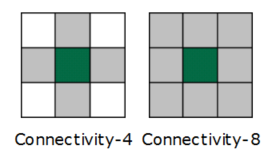
\includegraphics[width=0.4\textwidth]{images/connectivity.png}
  \caption{ภาพแสดงความแตกต่างระหว่าง 4-connectivity และ 8-connectivity ในการพิจารณาการเชื่อมต่อของพิกเซล \cite{ni_vision_connectivity}}
  \label{fig:connectivity}
\end{figure}

ในขั้นตอน preprocessing Connectivity สามารถนำมาใช้ในการวิเคราะห์โครงสร้างของวัตถุเบื้องต้น เช่น การตรวจสอบความต่อเนื่องของบริเวณที่สนใจ หรือการลบสัญญาณรบกวนที่ไม่เป็นส่วนหนึ่งของวัตถุหลัก ซึ่งช่วยให้ข้อมูลที่นำเข้าสู่โมเดลมีคุณภาพมากขึ้น

ในขณะเดียวกัน ในขั้นตอน post-processing Connectivity มีบทบาทสำคัญในการปรับปรุงผลลัพธ์ของการแบ่งส่วนภาพ โดยสามารถใช้ในการลบวัตถุขนาดเล็กที่ไม่เกี่ยวข้อง (small connected components removal) การรวมบริเวณที่ควรเป็นวัตถุเดียวกัน และการเติมช่องว่างภายในวัตถุ (hole filling) เพื่อให้ segmentation mask มีความสมบูรณ์และสอดคล้องกับลักษณะจริงของวัตถุมากยิ่งขึ้น

สำหรับโครงงานนี้ แนวคิดของ 8-connectivity ถูกนำมาใช้ในการวิเคราะห์วัตถุในภาพทั้งในขั้นตอน preprocessing และ post-processing เนื่องจากสามารถตรวจจับการเชื่อมต่อของพิกเซลได้ครอบคลุมมากกว่า 4-connectivity โดยเฉพาะในกรณีที่วัตถุมีลักษณะไม่เป็นระเบียบหรือมีขอบเขตที่ซับซ้อน ซึ่งช่วยปรับปรุงความถูกต้องของผลลัพธ์การแบ่งส่วนภาพได้อย่างมีประสิทธิภาพ


\section{Evaluation Metrics}
การประเมินประสิทธิภาพของแบบจำลองการแบ่งส่วนภาพ (image segmentation) มีความสำคัญในการวัดความสอดคล้องระหว่างผลลัพธ์ที่โมเดลทำนาย (prediction) และข้อมูลจริง (ground truth) โดยตัวชี้วัดที่นิยมใช้ ได้แก่ Precision, Recall, F1-score, Intersection over Union (IoU) และ Boundary F1 score ซึ่งสามารถสะท้อนประสิทธิภาพของโมเดลในมิติต่าง ๆ ได้อย่างครอบคลุม \cite{powers2011evaluation, everingham2015pascal}

\subsection{Precision}
Precision เป็นตัวชี้วัดที่ใช้วัดความถูกต้องของผลลัพธ์ที่โมเดลทำนายว่าเป็นวัตถุ โดยพิจารณาว่าพิกเซลที่ถูกทำนายว่าเป็นวัตถุ (positive) นั้นถูกต้องมากน้อยเพียงใด โดยคำนวณได้จากสูตร
\begin{equation}
\text{Precision} = \frac{TP}{TP + FP}
\end{equation}
โดยที่ $TP$ (True Positives) คือจำนวนพิกเซลที่ทำนายถูกต้อง, $FP$ (False Positives) คือจำนวนพิกเซลที่ทำนายผิดว่าเป็นวัตถุ 

Precision มีความสำคัญในกรณีที่ต้องการให้โมเดลมีความแม่นยำสูงในการทำนายวัตถุ โดยเฉพาะในงานที่การทำนายผิดอาจมีผลกระทบต่อการวิเคราะห์หรือการตัดสินใจ เช่น ในงานทางการแพทย์ที่การทำนายผิดอาจนำไปสู่การวินิจฉัยที่ไม่ถูกต้อง


\subsection{Recall}
Recall ใช้วัดความสามารถของโมเดลในการตรวจจับวัตถุทั้งหมด โดยพิจารณาว่าพิกเซลของวัตถุจริงถูกตรวจจับได้ครบถ้วนเพียงใด โดยคำนวณได้จากสูตร
\begin{equation}
\text{Recall} = \frac{TP}{TP + FN}
\end{equation}
โดยที่ $FN$ (False Negatives) คือจำนวนพิกเซลของวัตถุที่โมเดลไม่สามารถตรวจจับได้

Recall มีความสำคัญในกรณีที่ต้องการให้โมเดลสามารถตรวจจับวัตถุได้ครบถ้วน โดยเฉพาะในงานทางการแพทย์ที่การพลาดตรวจจับวัตถุอาจมีผลกระทบต่อการวินิจฉัยและการรักษา


\subsection{F1-score}
F1-score เป็นค่าเฉลี่ยแบบ harmonic mean ระหว่าง Precision และ Recall ซึ่งช่วยสร้างสมดุลระหว่างความแม่นยำและความครอบคลุมของโมเดล โดยคำนวณได้จากสูตร
\begin{equation}
\text{F1-score} = 2 \cdot \frac{\text{Precision} \cdot \text{Recall}}{\text{Precision} + \text{Recall}}
\end{equation}
F1-score เหมาะสำหรับกรณีที่ข้อมูลมีความไม่สมดุล (class imbalance) ซึ่งมักพบในงาน segmentation ทางการแพทย์ \cite{powers2011evaluation}


\subsection{Intersection over Union (IoU)}
Intersection over Union (IoU) หรือ Jaccard Index เป็นตัวชี้วัดที่ใช้วัดความซ้อนทับระหว่างพื้นที่ที่โมเดลทำนายและข้อมูลจริง โดยพิจารณาสัดส่วนของพื้นที่ที่ซ้อนทับกันต่อพื้นที่รวมของทั้งสอง โดยคำนวณได้จากสูตร
\begin{equation}
\text{IoU} = \frac{TP}{TP + FP + FN}
\end{equation}
IoU เป็นตัวชี้วัดที่นิยมใช้ในงาน segmentation เนื่องจากสามารถสะท้อนความแม่นยำของการแบ่งส่วนภาพได้อย่างชัดเจน โดยเฉพาะในกรณีที่ต้องการประเมินความสอดคล้องของขอบเขตวัตถุกับข้อมูลจริง \cite{everingham2015pascal}


\subsection{Boundary F1 Score}
Boundary F1 Score เป็นตัวชี้วัดที่ใช้ประเมินความถูกต้องของขอบเขต (boundary) ของวัตถุ โดยมุ่งเน้นไปที่ความสอดคล้องของเส้นขอบระหว่าง prediction และ ground truth ซึ่งมีความสำคัญในงาน segmentation ที่ต้องการความละเอียดสูง เช่น ภาพทางการแพทย์ \cite{cheng2021boundary}

แนวคิดของ Boundary F1 คือการพิจารณา Precision และ Recall เฉพาะบริเวณขอบของวัตถุ โดยใช้ระยะ tolerance ในการกำหนดว่าขอบที่ทำนายใกล้เคียงกับขอบจริงมากเพียงใด ซึ่งช่วยให้สามารถประเมินคุณภาพของ segmentation ในบริเวณที่มีความสำคัญสูงได้ดียิ่งขึ้น \newline

ในโครงงานนี้ ได้เลือกใช้ตัวชี้วัดหลายประเภทเพื่อให้สามารถประเมินประสิทธิภาพของโมเดลได้อย่างครอบคลุม โดย Precision, Recall และ F1-score ใช้ในการประเมินความถูกต้องของการจำแนกพิกเซล ขณะที่ IoU ใช้ในการวัดความสอดคล้องเชิงพื้นที่ และ Boundary F1 ใช้ในการประเมินความแม่นยำของขอบเขตของอวัยวะ

การใช้ตัวชี้วัดหลายรูปแบบร่วมกันช่วยให้สามารถวิเคราะห์จุดแข็งและข้อจำกัดของโมเดลได้อย่างละเอียด โดยเฉพาะในกรณีที่ผลลัพธ์มีความคลาดเคลื่อนบริเวณขอบวัตถุ หรือมีปัญหา class imbalance ซึ่งสอดคล้องกับลักษณะของข้อมูลภาพช่องปากที่ใช้ในการทดลอง



% \section{\ifenglish%
% \ifcpe CPE \else ISNE \fi knowledge used, applied, or integrated in this project
% \else%
% ความรู้ตามหลักสูตรซึ่งถูกนำมาใช้หรือบูรณาการในโครงงาน
% \fi
% }

% อธิบายถึงความรู้ และแนวทางการนำความรู้ต่างๆ ที่ได้เรียนตามหลักสูตร ซึ่งถูกนำมาใช้ในโครงงาน

% \section{\ifenglish%
% Extracurricular knowledge used, applied, or integrated in this project
% \else%
% ความรู้นอกหลักสูตรซึ่งถูกนำมาใช้หรือบูรณาการในโครงงาน
% \fi
% }

% อธิบายถึงความรู้ต่างๆ ที่เรียนรู้ด้วยตนเอง และแนวทางการนำความรู้เหล่านั้นมาใช้ในโครงงาน
